% Capítulo 4
\chapter{Arquitetura}
\label{ch:architecture}

A robótica tenta solucionar problemas envolvendo diversas áreas da computação. Desde o controle de motores, usando programação de baixo nível, até soluções sofisticas utilizando \abrv[IA -- Inteligência artificial]{IA (Inteligência artificial)} aplicada a visão e tomada de decisões, entre outros. Assim, o desenvolvimento de uma única ferramenta, em uma única linguagem, que solucione todos os problemas pode tornar-se impraticável o estágio atual da tecnologia, já que as linguagens são projetadas com intenções e problemas diferentes em mente.

Para solucionar este problema, a arquitetura adotada pelo time AUT-UofM é distribuída, baseada no \textit{framework} ROS. Onde cada componente tem uma função diferente dentro do sistema total. O ROS é uma coleção de bibliotecas e convenções para simplificar a tarefa de criar comportamentos complexos na grande variedade de robôs e suas plataformas \cite{ros2017}.

Desta forma, este capítulo divide cada subsistema dentro do robô como componentes apresentando suas funções antes e após implementadas as mudanças propostas pelo trabalho em suas diferentes camadas de execução. Alguns deles são mais detalhados e descritos em seus módulos, apresentando alguns fluxogramas e diagramas afim de expressar melhor seu funcionamento.

\section{Componentes e arquitetura atual}
\label{sec:architecture:current_components_and_architecture}

A arquitetura do sistema pode ser abstraída em $3$ camadas: A camada de \textit{hardware}, a de software de baixo nível, e a de software.

Na camada de \textit{hardware}, a mais inferior na figura~\ref{fig:softwarearchitecture:overview}, estão contidos os componentes físicos do sistema. Uma câmera \textit{Webcam Logintech C920 Pro HD 15MP Full HD1080p} é usada para fornecer imagens para o sistema de visão. Uma \abrv[IMU -- do inglês \textit{Inertia Measurement Unit}]{\textit{IMU}}, do inglês \textit{Inertia Measurement Unit}, é usada para fornecer informações para o posterior cálculo da orientação do corpo do robô em relação ao eixo de gravidade. E os motores, também chamados de atuadores, são utilizados nas juntas para os movimentos às partes do robô.

A camada de software de baixo nível é responsável pelo processamento de dados da \textit{IMU}, juntamente com a execução do \textit{walking gait}. Esta camada roda dentro da placa microcontroladora \textit{Robotis.Co OpenCM9.04}, ou simplesmente \textit{OpenCM9.04}.

A placa controladora conta com um processador \textit{32bit ARM Cortex-M3}, memória \textit{flash} (que mantém os dados mesmo quando desligada) de 128Kb e 20Kb de \textit{SRAM} \cite{opencm904}. A placa tem seu projeto e código fonte abertos e foi utiliza a \textit{Arduino IDE} como \abrv[IDE -- do inglês \textit{integrated development environment}]{IDE} de desenvolvimento. Ela conecta-se ao controlador principal via USB, por onde há troca de dados. Adicionalmente, devido ser produzida pela mesma empresa, a placa integra-se perfeitamente com os motores utilizados no projeto de Arash.

Os motores, todos pertencentes a categoria \textit{Dynamixel}, são atuadores inteligentes otimizados para robôs. Eles possuem controle \abrv[PID -- do inglês \textit{Porportional Integral Derivative}]{PID} integrado e comunicar-se em uma rede de comunicação \abrv[TTL -- Do inglês \textit{transistor-transistor logic}]{TTL (\textit{transistor-transistor logic})}{} com \textit{baudrate} de até $4.5$ Mbps \cite{dynamixel}.

A camada de software é executada dentro de um computador, doravante referido como controlador principal, \textit{mini-box PC MAXData QutePC-3001} com um processador 64 bits de dois núcleos Intel\copyright{} Celeron\copyright{} 847E (1,1GHz e 2MB de \textit{cache}), rodando o sistema operacional Linux Ubuntu versão 14.04. Esta camada é responsável por rodar os componentes de software, de alto nível, e enviar comandos de controle para a camada inferior, de baixo nível -- figura~\ref{fig:softwarearchitecture:overview}.

\begin{figure}[htb]
	\centering
	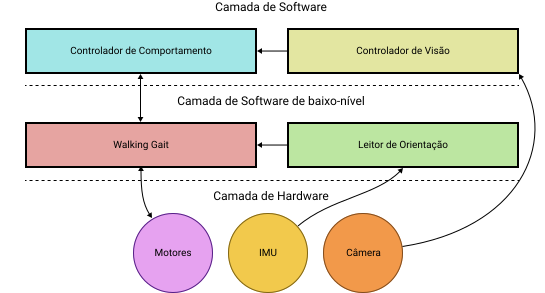
\includegraphics[scale=1]{imagens/svg/softwarearchitecture-flow}
	\caption{Fluxograma simplificado da arquitetura atual e seus fluxos.}
	\label{fig:softwarearchitecture:overview}
\end{figure}

A figura~\ref{fig:softwarearchitecture:overview} mostra uma visão simplificada dos principais componentes -- e o sentido do fluxo de dados entre eles -- envolvidos no processo de uma tarefa genérica hipotética. O funcionamento de cada componente individual será detalhado nas próximas seções.

\subsection{Visão}

Visão não é o foco deste trabalho. Entretanto, uma explanação geral é necessária afim de melhor entender o funcionamento geral do sistema.

\begin{figure}[h!]
	\centering
	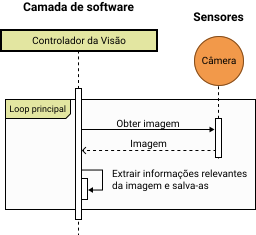
\includegraphics[scale=1]{imagens/svg/softwarearchitecture-vision}
	\caption{Diagrama de sequência simplificando do \textit{loop} principal do componente de visão.}
	\label{fig:softwarearchitecture:vision}
\end{figure}

O controle de visão é um software que conecta-se via USB com a câmera, analisando as imagens e extraindo informações relevantes à execução da tarefa do robô. De forma geral, podemos abstrair seu funcionamento em duas \textit{threads} distintas:

A primeira é o \textit{loop} principal, representada no diagrama de sequência na figura \ref{fig:softwarearchitecture:vision}. Em um primeiro passo, o controlador obtém a imagem da câmera. Em seguida, a extração de informações é realizada. Essas informações dependem da tarefa que o robô deve realizar. Por exemplo, detectar a bola, os adversários e as linhas do campo, em caso de da tarefa ser uma partida de futebol; ou detectar as linhas guia da pista de corrida no caso da tarefa ser uma corrida. Em seguida, tudo o que foi encontrado é salvo para futuras consultas até que a próxima iteração ocorra e os dados sejam atualizados.

A segunda \textit{thread}, cuja a interação pode ser visualizada na figura~\ref{fig:softwarearchitecture:software}, do controle de visão executa o sistema de comunicação que pode ser implementado de várias maneiras, desde objetos \textit{JSON} sendo transmitidos via \textit{UDP} até um \textit{message broker} com filas de consumo. Ao receber a mensagem de solicitação das informações, responde serializando os dados que ficaram salvos na primeira \textit{thread}, fornecendo as informações com atraso mínimo.

Neste trabalho, nenhuma implementação relacionada a visão foi produzida.

\subsection{Controlador de Comportamento}

O controlador de comportamento roda na camada de \textit{software} e implementa a tarefa que deve ser realizada pelo robô. Ele funciona como um gerente que coordena outros componentes, recebendo informações e enviando comandos com ações específicas serem a executadas. Na figura~\ref{fig:softwarearchitecture:software} é possível observar a sequência de passos realizados pelo controlador de comportamento.

Usando como exemplo uma partida de futebol, na figura~\ref{fig:softwarearchitecture:software} observa-se o controlador de comportamento ``jogador'' consultando o componente de visão, que responde a posição da bola, previamente obtida durante o processo da figura~\ref{fig:softwarearchitecture:vision}. Em seguida, baseado nessas informações o comportamento envia o comando ao \textit{walking gait} para caminhar na direção correta.

Normalmente este processo é contínuo. A detecção é realizada, as informações são processadas, a decisão é tomada, o comando é enviado e o sistema aguarda o início da próxima iteração, onde tudo será repetido.

\begin{figure}[htb]
	\centering
	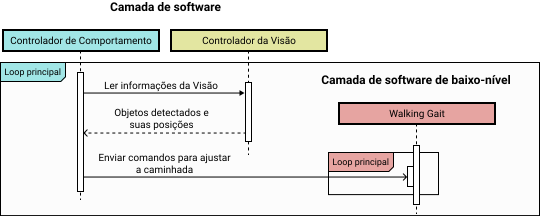
\includegraphics[scale=1]{imagens/svg/softwarearchitecture-software}
	\caption{Diagrama de sequência do controlador de comportamento e suas dependências.}
	\label{fig:softwarearchitecture:software}
\end{figure}

\subsection{\textit{Walking Gait} e Leitor de Orientação}

O componente \textit{walking gait} coordena e executa a caminhada. Ele monitora a USB aguardando os comandos de controle que contém as velocidades da caminhada, enviados a partir do controlador de comportamento.

O componente leitor de orientação desempenha um papel importante ao lado do \textit{walking gait}. Ele é o responsável pela verificação da orientação da rotação do torso -- uma vez que a \textit{IMU} está situada nas costas de Arash -- assim fornecendo dados para o \textit{walking gait} fazer correções durante a caminhada afim de compensar um eventual distúrbio.

\begin{figure}[htb]
	\centering
	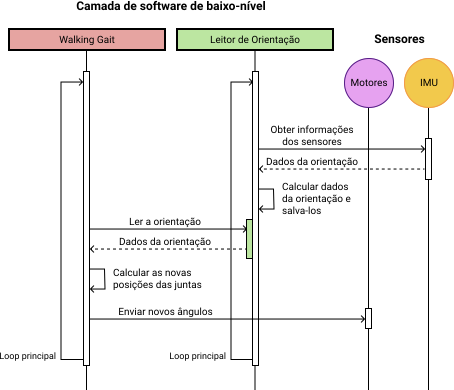
\includegraphics[scale=0.8]{imagens/svg/softwarearchitecture-lowlevel}
	\caption{Diagrama de sequência simplificando do \textit{walking gait} e do leitor de orientação.}
	\label{fig:softwarearchitecture:lowlevel}
\end{figure}

Ainda no leitor de orientação, os dados são coletados da \textit{IMU} e um processo de utilizando filtro de \textit{Kalman} é utilizado para obter uma estimativa mais acurada das orientações que são salvas em variáveis. Já na \textit{thread} que roda o \textit{walking gait}, a orientação é continuamente consultada e utilizada para que os ângulos das juntas sejam atualizados. O filtro de Kalman é um algoritmo que -- dada uma séria de observações no tempo e suas incertezas -- é capaz de, estatisticamente, calcular um valor que tende a ser mais próximo ao real \cite{grewal2014}.

Dentro da placa microcontroladora \textit{OpenCM9.04}, o \textit{walking gait} e o leitor de orientação rodam em \textit{threads} dinstintas, recurso este habilitado pela biblioteca \textit{MapleFreeRTOS}. Na figura~\ref{fig:softwarearchitecture:lowlevel} observa-se a execução de ambas a \textit{threads} separadamente e a forma de interação entre elas. Iniciando a partir do \textit{walking gait}, onde os dados de orientação são lidos diretamente do leitor de orientação, em seguida calcula-se os ângulos das juntas que são enviadas aos motores. Em paralelo, o leitor de orientação continua recebendo os dados da \textit{IMU}, processando e salvando-os para que fiquem disponíveis ao \textit{walking gait}. Nota-se que, em ambas as \textit{threads}, as sequências de ações são executadas dentro de \textit{loops} principais.

Para sumarizar, foram apresentados os componentes, da arquitetura atual, e o seu papel dentro do sistema completo. Seus fluxos de dados e uma base de como seu processamento ocorre também foi mostrado.

\section{A nova arquitetura}

De acordo com os problemas e solução já discutidos em seções anteriores, esta seção irá apresentar as mudanças realizadas na arquitetura original apresentada na seção~\ref{sec:architecture:current_components_and_architecture}.

Uma das principais mudanças realizadas neste trabalho é a re-implementação do \textit{walking gait}. Nessas modificações ainda faz-se necessário a a utilização da \textit{OpenCM9.04}. Entretanto, ela assume o papel de reencaminhar os dados dos ângulos aos motores e, ainda, fornecer os dados de orientação ao \textit{walking gait}.

\begin{figure}[h!]
	\centering
	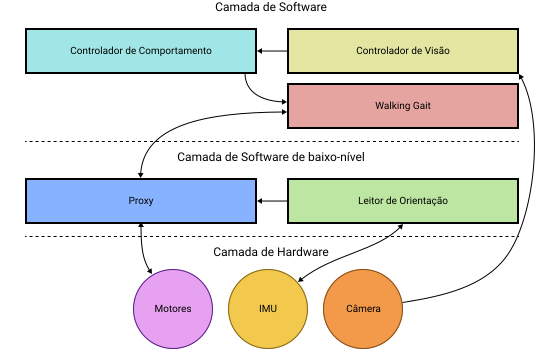
\includegraphics[scale=1]{imagens/svg/softwarearchitecture-newproposal}
	\caption{Fluxograma simplificado da nova arquitetura e seus fluxos de dados.}
	\label{fig:softwarearchitecture:newproposal}
\end{figure}

A figura~\ref{fig:softwarearchitecture:newproposal} mostra a visão simplificada da nova arquitetura. Nela observa-se o \textit{walking gait} -- agora na camada de \textit{software} -- funcionando dentro do controlador principal, e um novo componente chamado \textit{proxy} é apresentado como interface os componentes de \textit{hardware} e o \textit{walking gait}. O papel do novo componente é de servir realmente como um \textit{proxy} enviando comandos recebidos do controlador principal aos motores e também receber a orientação do componente leitor de orientação e fornecê-la ao controlador principal.

O controlador de comportamento continua a enviar os comandos de controle ao \textit{walking gait}. Porém, ao invés de usar comandos binários via USB, agora utiliza objetos serializados via \abrv[JSON -- \textit{Java Script Object Notation}]{JSON}{}por UDP (seção~\ref{subsec:architecture:walkinggait:controlserver}).

Entre o \textit{walking gait} e o \textit{Proxy} a comunicação ocorre via USB @ 1 Mbps. Comandos de controle utilizando o \textit{dynamixel protocol 2.0} são gerados e enviados diretamente do \textit{walking gait} ao \textit{Proxy}, que apenas os encaminha aos motores. Esta estratégia foi adotada para habilitar a possibilidade da utilização de motores de diferentes tipos, não apenas da Robotis Co. Assim, apenas o \textit{walking gait} é responsável pela geração de destes comandos específicos de cada motor enquanto o \textit{Proxy} apenas os encaminha.

Na camada de \textit{software} de baixo nível, o leitor de orientação continua a fornecer os dados de orientação. Porém, ao invés do \textit{walking gait} acessá-los diretamente, o \textit{Proxy} encarrega-se de disponibiliza-los ao \textit{walking gait}.

\begin{figure}[h!]
	\centering
	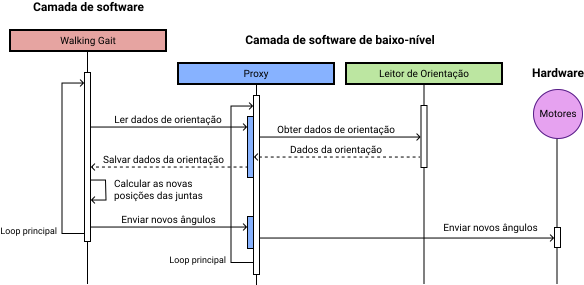
\includegraphics[scale=1]{imagens/svg/softwarearchitecture-newproposal-sequence}
	\caption{Diagrama de sequência simplificado mostrando a interação entre o \textit{walking gait} e os componentes de baixo nível.}
	\label{fig:softwarearchitecture:newproposal:sequence}
\end{figure}

Na figura~\ref{fig:softwarearchitecture:newproposal:sequence}, é possível observar o diagrama de sequência com os componentes que foram atingidos pela mudança na arquitetura. O \textit{walking gait} lê os dados de orientação, calcula as novas posições das juntas e envia os novos ângulos ao \textit{Proxy} e processo volta ao início. Enquanto isso, o \textit{Proxy} obtém os dados de orientação diretamente do Leitor de orientação, em seguida os fornece ao \textit{walking gait}.

\section{\textit{Walking gait}}

A nova implementação do \textit{walking gait}, uma mudança completa paradigma estruturado ao orientado a objetos foi realizada. Afim de facilitar o desenvolvimento, o projeto foi divido em $3$ submódulos: o servidor de controle, o motor de caminhada e o atualizador de juntas.

Nesta seção, os três submódulos são apresentados e,  por fim, um software de apoio chamado visualizador 3D é apresentado.

Adicionalmente, todos os parâmetros de configuração -- tais como as portas do de controle do visualizador 3D e servidor de controle (descritos nas próximas seções), deslocamentos físicos das juntas (\textit{offsets}), peso de compensação do processo de  \textit{swing} do corpo ($B_{swing}$), a frequência de geração dos moimentos ($Gait_{frequency}$), o \textit{walking gait} possui um esquema de configurações baseado em objetos JSON salvos em arquivos. Desta forma, é possível inicializar o componente com diversas parâmetros diferentes. Assim, também é possível o versionamento dos arquivos de configuração, para que alterações sejam mantidas de forma rastreável.

\subsection{Servidor de controle}
\label{subsec:architecture:walkinggait:controlserver}

O servidor de controle é um submódulo que é implementa a interface de comunicação do \textit{walking gait} a outros componentes do sistema. De fato, todo o gerenciamento da caminhada pode ser realizada a partir de um único comando que atualizam as velocidades $V_x$, $V_y$ e $V_\theta$.

\begin{figure}[htb]
	\begin{lstlisting}[language=json,firstnumber=1]
{
  "command": "omniwalk",
  "params":
  {
    "x": 0.3, // Opcional: Velocidade no eixo X
    "y": 0.6, // Opcional: Velocidade no eixo Y
    "theta": 0.0  // Opcional: Velocidade no eixo teta
  }
}
	\end{lstlisting}
	\caption{Comando de controle exemplo, em JSON.}
	\label{fig:architecture:walkinggait:controller:json}
\end{figure}

Para tal tarefa, adotou-se uma solução simplista que consiste em receber objetos serializados \textit{JSON} através de um servidor \textit{UDP}, principalmente por causa de sua rápida implementação.

Sabe-se que o protocolo UDP não garante a integridade, nem a ordem, da entrega dos dados. Todavia, a aplicação inteira roda dentro da rede de \textit{loopback} dispensa essa preocupação. Também, como o processo é iterativo, caso alguma falha ocorra em uma iteração, ela logo será corrigida na próxima iteração. Adicionalmente, para esta aplicação, a não verificação dos pacotes pelo protocolo UDP, reverte-se em vantagem, já que não há o atraso de tempo necessário para sincronizar as duas pontas da comunicação. Além disso, esta abordagem aproveita-se da filosofia \textit{zero-copy} adotada pelo \textit{kernel} do Linux \cite{tianhua2008} que evita fazer cópia dos \textit{buffers} das mensagens recebidas via rede, desde o \textit{driver} de rede até a entrega na aplicação.

Na figura~\ref{fig:architecture:walkinggait:controller:json} observa-se um comando de controle JSON. A propriedade \textit{command} que identifica a intenção do comando de alterar os parâmetros da caminhada. A propriedade \textit{params} indica um sub-objeto \textit{JSON} com as propriedades \textit{x}, $y$ e $theta$ representanto, respectivamente, $V_x$, $V_y$ e $V_\theta$. Todas as propriedades são opcionais, e caso não sejam informadas, nenhuma modificação será feita naquele eixo faltante.

Em caso de intenção de parada, o mesmo comando \textit{omniwalk} deverá ser enviado porém com todas as velocidades com valor $0.0$.

\subsection{Motor de caminhada}

O motor de caminhada é o submódulo onde os processos dos cálculo das trajetórias, e da IK serão executados e guardados para, posteriormente, serem aplicados aos motores pelo submódulo atualizador de juntas (subseção \ref{subsec:architecture:walkinggait:jointsupdater}).

A classe $Humanoid$ é usada para a manter o estado das juntas, tanto posição quanto angulações. Ela também é usada para manter os estados das juntas durante os cálculos da \textit{IK}.

\begin{figure}[htb]
	\centering
	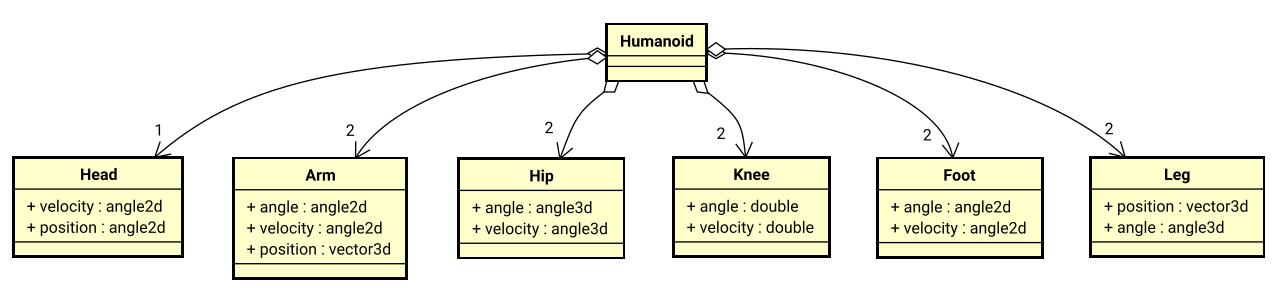
\includegraphics[scale=0.4]{imagens/svg/walkinggait-domain}
	\caption{Diagrama de domínio do \textit{walking gait}.}
	\label{fig:architecture:walkinggait:domain}
\end{figure}

A figura~\ref{fig:architecture:walkinggait:domain} mostra o diagrama de domínio das classes mais relevantes aos dados que o componente manipula. Observa-se todas as composições envolvidas na definição da classe $Humanoid$, que representa todo o conjunto das juntas de Arash. Também, nota-se que nas classes $Head$, $Arm$, $Hip$, $Knee$, $Foot$ existem dados de ângulo e velocidade. Isso dá-se por causa que componente utiliza essas informações para calcular o próximo estado do sistema em caso de algum distúrbio. Também, a classe $Leg$ aparece de forma ambígua, já que existem as definições de $Hip$, $Knee$ e $Foot$. Porém, a classe $Leg$, representa os dados da cinemática inversa de uma perna, enquanto as demais classes guardam o estado atual das partes que representam.

Ainda na figura~\ref{fig:architecture:walkinggait:domain}, a notação dos dados utilizados: $angle2d$, $angle3d$ e $vector3d$. Estes tipos possuem o sufixo numérico, que indica a quantidade de dimensões aquela classe guarda, e a letra, que indica o tipo de dado, no caso $d$ é referente a $double$. Para ângulos, $2$ dimensões significa que os eixos de rotação $pitch$ e $roll$ são guardados; já os ângulos com $3$ eixos, as orientações $roll$, $pitch$ e $yaw$ são guardadas. Para vetores, os valores nas dimensões $x$, $y$ e $z$ são mantidos.

O processo de caminhada inicia-se no momento em que qualquer velocidade é diferente de zero. Quando isso ocorre (ou seja, um comando de controle é recebido), a instância da classe $Robot$, doravante referida apenas como $robot$, através de seu método $omniGait$, faz uma interpolação linear entre a velocidade atual e a nova velocidade. A medida que a velocidade é gradualmente alterada para seu novo valor, o relógio central é iniciado e o método $updateTrajectories$ é chamado, calculando a trajetória (de acordo com a seção \ref{sec:math:trajectories}) e guardando-a na variável de instância $humanoid$, do tipo $Humanoid$. Enfim, o método $update$ de $Ik$ é chamado para que execute os cálculos da cinemática inversa. O diagrama de sequência simplificado na figura~\ref{fig:architecture:walkinggait:walkengine:sequence} mostra este processo.

\begin{figure}[htb]
	\centering
	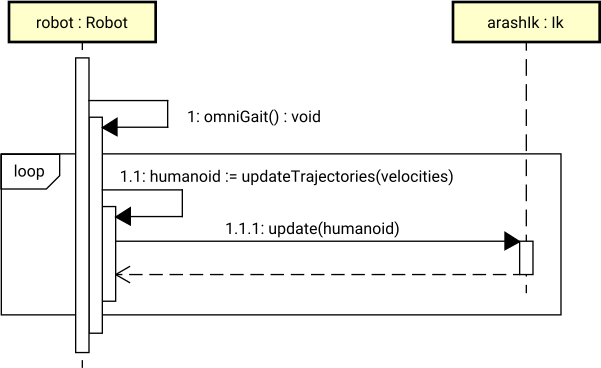
\includegraphics[scale=0.5]{imagens/svg/walkinggait-walkingengine-sequence}
	\caption{Diagrama de sequência simplificado do motor de caminhada.}
	\label{fig:architecture:walkinggait:walkengine:sequence}
\end{figure}

\subsection{Atualizador de juntas}
\label{subsec:architecture:walkinggait:jointsupdater}

Este módulo é responsável pela atualização dos ângulos dos motores. Ele roda em sua própria \textit{thread}, afim de não bloquear o processamento dos demais componentes do \textit{walking gait}.

A implementação base do atualizador de juntas, usa uma abstração de motores afim de prover a possibilidade do uso de motores de fabricantes diferentes em futuras aplicações.

\begin{figure}[htb]
	\centering
	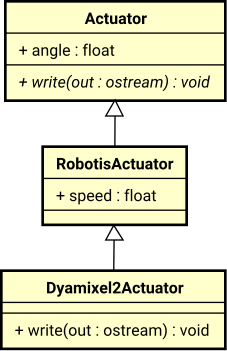
\includegraphics[scale=0.6]{imagens/svg/softwarearchitecture-actuators-hierarchy}
	\caption{Fragmento do diagrama de classe da hierarquia dos atuadores.}
	\label{fig:architecture:actuator:classdiagram}
\end{figure}

A classe abstrata $Actuator$, base da implementação dos atuadores, define a propriedade de posição, referida na classe como $angle$, comum a todos os atuadores. Cada tipo de atuador, pode ter diferentes características e parâmetros de acordo com seu fabricante, embora todos tenham o mesmo objetivo.

Construída sobre a classe $Actuator$ está a classe $Dynamixel2Actuator$. Ela adiciona as propriedades $id$ e $speed$. O $id$ é a identificação numérica de cada junta, solução adotada pela Robotis para identificar cada atuador dentro da rede TTL. Já a $speed$ é a velocidade que a posição é alcançada. Todos os atuadores utilizados em Arash funcionam usando o mesmo protocolo, apesar das diferentes versões. Assim, todos são representados por instâncias desta classe.

A figura~\ref{fig:architecture:actuator:classdiagram} mostra o diagrama de classe com a hierarquia e os principais métodos e propriedades das classes $Actuator$ e $Dynamixel2Actuator$.

A classe $ActuatorUpdater$ implementa uma iteração completa do processo de atualização das juntas e a figura~\ref{fig:architecture:actuatorupdater:sequence} mostra este processo. Para mante-lo rodando continuamente, uma \textit{thread} mantém o método $update$ sendo chamando continuamente. A frequência de atualização é sincronizada com a geração dos dados pelo módulo do motor de caminhada.

\begin{figure}[htb]
	\centering
	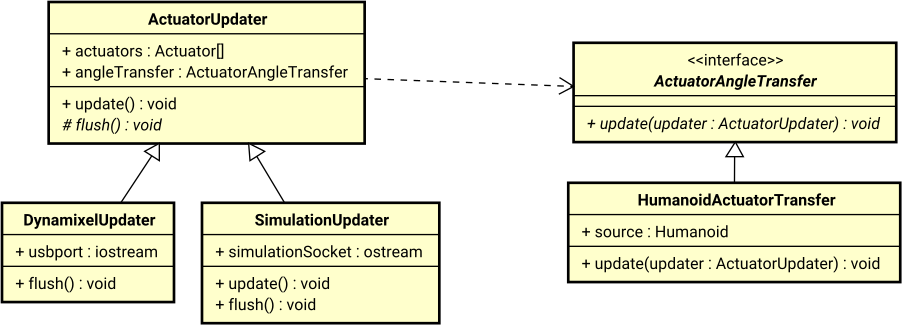
\includegraphics[scale=0.6]{imagens/svg/softwarearchitecture-actuatorupdater-classdiagram}
	\caption{Fragmento do diagrama de classe da hierarquia dos atualizadores de atuadores.}
	\label{fig:architecture:actuatorupdater:classdiagram}
\end{figure}

Na figura~\ref{fig:architecture:actuatorupdater:classdiagram} é possível observar as principais classes envolvendo o processo de atualização. A classe $ActuatorUpdater$ é responsável por enviar os dados calculados pelo motor de caminhada aos atuadores. Porém, ela é uma classe abstrata e serve apenas como implementação básica para as reais implementações. A classe concreta $DynamixelUpdater$, filha de $ActuatorUpdater$, define o método $flush$ implementando os comandos \textit{Dynamixel 2.0} \cite{dynamixel} para os motores reais. A classe concreta $SimulationUpdater$, também filha de $ActuatorUpdater$, implementa a comunicação para um sistema de visualização, descrito nas próximas seções, que habilita a visualização dos movimentos do robô usando um ambiente 3D facilitando a visualização dos movimentos.

Pensando em futuras implementações, criou-se a classe abstrata $ActuatorAngleTransfer$ que é responsável por conhecer a estrutura do robô e quais atuadores são as equivalentes as juntas. Assim, quando seu método $update$ é chamado, este transfere todos os ângulos das juntas, situados em sua propriedade $source$, às suas respectivas instâncias de $Actuator$ correspondentes. A propriedade $source$ é uma instância da classe $Humanoid$ que é atualizada pelo motor de caminhada ao final do processamento da sua iteração.

Acompanhando o diagrama de sequência da figura~\ref{fig:architecture:actuatorupdater:sequence}, podemos ver o método $update$ de $ActuatorUpdater$ sendo chamado. Na sequência, o método $update$ de \textit{humanoidAngleTransfer} é chamado passando a própria instância de $ActuatorUpdater$, onde todos os dados das juntas são transferidos de $source$ (propriedade de \textit{humanoidAngleTransfer}) para os atuadores contidos na propriedade $actuators$ de $updater$. Assim, finalmente, sendo chamado o método $flush$ de $ActuatorUpdater$ que implementa a verdadeira comunicação com o motor.

\begin{figure}[htb]
	\centering
	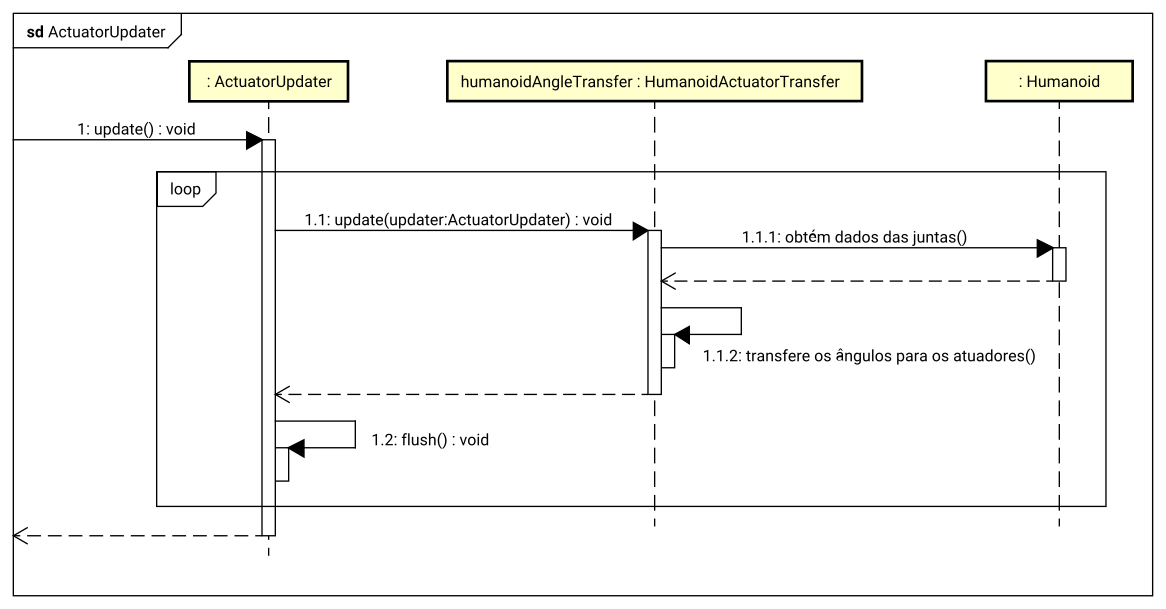
\includegraphics[scale=0.45]{imagens/svg/softwarearchitecture-actuatorudpater-sequence}
	\caption{Fragmento do diagrama de classe da hierarquia dos atuadores.}
	\label{fig:architecture:actuatorupdater:sequence}
\end{figure}

Retornando à figura~\ref{fig:architecture:actuatorupdater:classdiagram} observa-se duas implementações de $ActuatorUpdater$. A primeira implementação, a classe $Dynamixel2Updater$, implementa o protocolo \textit{Dynamixel 2.0} e faz a comunicação via USB com o componente \textit{Proxy}. Após os dados serem enviados ao \textit{Proxy}, este encaminhará os dados aos motores que executam o comando posicionando as juntas.

A segunda implementação, a classe $SimulationUpdater$, envia as informações do atuador ao visualizador 3D. Ao envio é realizado através da serialização das informações em um objeto JSON e transmitido via UDP, de forma similar ao servidor de controle implementado no \textit{walking gait}.

A figura~\ref{fig:architecture:walkinggait:visualization:json} mostra um pacote de atualização de exemplo com as propriedades das juntas e seus ângulos. Nota-se a propriedade \textit{params} com um objeto JSON com suas chaves definindo os nomes das juntas recebendo outros objetos com a propriedade \textit{angle} com o valor dos ângulos em radianos.

\begin{figure}[htb]
	\begin{lstlisting}[language=json,firstnumber=1]
{
  "command": "update",
  "params":
  {
    "RightHipLateral": { "angle": 0.1 },
    "RightHipTransversal": { "angle": 0.2 },
    "RightHipFrontal": { "angle": 0.3 },
    "RightKneeLateral": { "angle": 0.4 },
	...,
    "LeftFeetLateral": { "angle": 0.5 },
    "LeftFeetFrontal": { "angle": 0.6 }
  }
}
\end{lstlisting}
	\caption{Comando de controle recebido pelo visualizador 3D.}
	\label{fig:architecture:walkinggait:visualization:json}
\end{figure}

\subsection{Visualizador 3D}

As trajetórias geradas, juntamente com os 20 ângulos radianos das juntas, gerados pelo \textit{walking gait} são difíceis de visualizar e validar. Desta forma torna-se necessária uma forma de visualizar, mesmo que de forma preliminar, o resultado; já que o acesso ao robô de forma física é impossível.

\begin{figure}[htb]
	\centering
	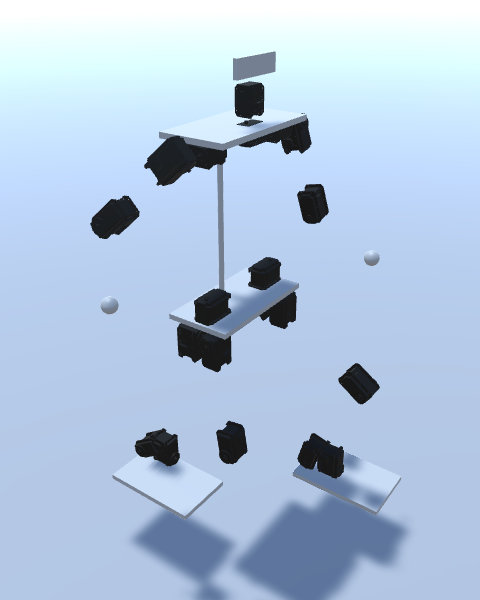
\includegraphics[scale=0.55]{imagens/visualizador3d}
	\caption{Captura de tela da imagem gerada pelo visualizador 3D.}
	\label{fig:architecture:visualization:printscreen}
\end{figure}

A melhor solução seria a utilização de um \textit{framework} de simulação, como Gazebo \cite{gazebo}. Onde seria possível validar toda o processo de caminhada. Todavia, por restrição de tempo impossibilitaram a adotação desta solução. 

Desta forma, o visualizador 3D é uma ferramenta de apoio ao desenvolvimento criada com o objetivo de habilitar a interpretação visual dos ângulos e trajetórias gerados pelo \textit{walking gait}.

Desenvolvido utilizando \textit{framework} Unity 3D 5.1, comumente utilizado para desenvolvimento de jogos, o visualizador 3D possui a estrutura de Arash em uma cadeia de atuadores anexadas para simular as rotações geradas pelo \textit{walking gait}. Entretando, sem efeitos físicos habilitados.

A comunicação entre o visualizador 3D e o \textit{walking gait} é realizada pela troca de \textit{JSON} via UDP, de forma similar ao servidor de controle (subseção~\ref{subsec:architecture:walkinggait:controlserver}). Cada pacote contém o estado completo de todas as juntas de Arash.

Ao receber os dados, o visualizador procura o atuador virtual correspondente e aplica a transformação na cadeia anexada a ele. A sequência de processo no tempo causa o efeito de animação.